\section{Results}
\label{sec:results}
\begin{figure}[h!]
\centering
	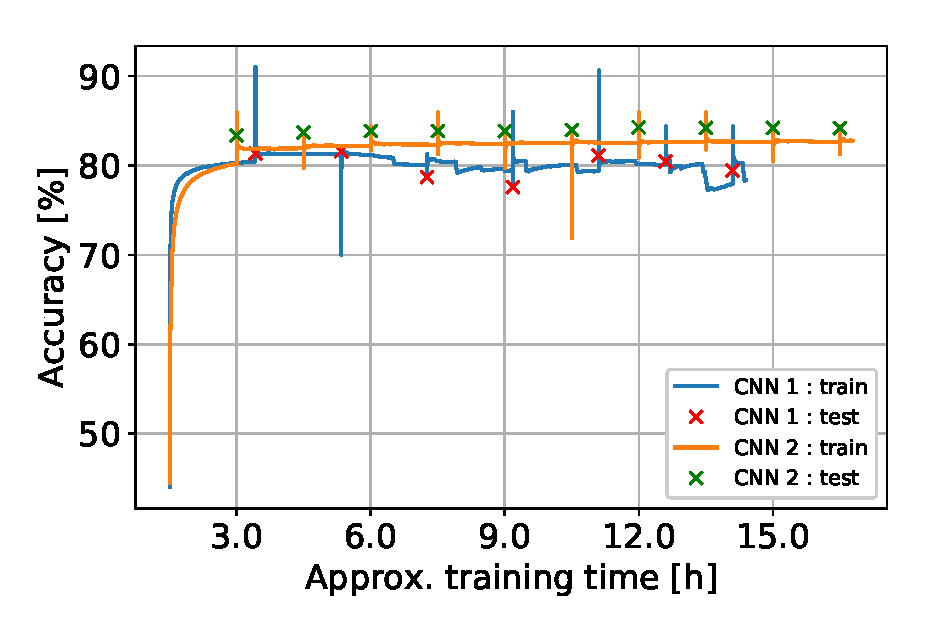
\includegraphics[scale=0.6]{CNNaccuracy} 
\caption{Training of the two convolutional neural nets. The first one does not use ``dropout'' as opposed as the second one.}
\label{plot:CNNaccuracy}
\end{figure}
\FloatBarrier


\begin{table}[h]
  \centering
  \begin{tabular}[c]{lllll}
    Input format&Model&Precision&Recall&Accuracy\\
    \hline
    Tweet-embed.&Logistic regression & 0.00       & 0.00  & 0.00 \\
    Tweet-embed.&SVM                 & 0.00       & 0.00  & 0.00 \\
    Tweet-embed.&Neural network	& 0.00	& 0.00	&	0.00 \\
    Word-embed.&CNN w.o. dropout                & 0.00	& 0.00	&	0.00 \\
    Word-embed.&CNN w. dropout & 0.00 & 0.00 & 0.00
    
  \end{tabular}
  \caption{Classification performances using local hold-out testing, for various input data formats.}
  \label{tab:results}
\end{table}


